\chapter{Robot Operating System}\label{c:ros}

As aforementioned, this thesis aims to explore the security configuration within Robot Operating System 2 (ROS2) and its security toolset Secure Robot Operating System 2 (SROS2), enabling the specification and model checking using Alloy. 

This chapter presents a detailed introduction to the concepts around Robot Operating System (ROS), as well as the evolution approach that ROS faced towards providing security to its deployed systems. Regarding this goal, Data Distribution Service (DDS) and its integration on Robot Operating System 2 (ROS2) must be contextualized beforehand. Thereafter, it will be presented a section dedicated to related work regarding the study of security in ROS based systems.

\section{Background}\label{s:ros-back}

Robotic systems have emerged into several scenarios, where its usage ranges between basic processes automation, up to full performance over critical tasks, consequently causing the complexity increase in these domains. Concerning the complexity behind writting software code, due to the widely variety presented in the robot's hardware as in fields of action, Robotic Operation System (ROS) presents itself as a middleware system, created to facilitate robotic systems development.

In ROS, software flexibility was valued above all else, meaning that values like security were not considered as a priority, so ROS-based applications tend to face increased security risks, compromising the whole robotic network. As ROS became a standard for many robotic systems, and due to the scale and scope of the robotics grows as they start to be integrated into the real world, security matters must be addressed as priority while developing systems involving robots. \cite{diluoffo2018robot, kim2018security}

The upgraded version of ROS, Robot Operating System 2 (ROS), presents itself as a framework for developing robotic systems, supported by a standard, the Data Distribution Service (DDS), where multiple middleware implementations are built over this standard, providing ROS applications multiple DDS-based specfications, as well as valued Quality of Service (QoS) settings over the transport configuration. 

The DDS-Security specification \cite{ros-dds-integration}, embedded by every DDS implementation supported by ROS, supplies multiple plugins regarding the security domain. As result, ROS2 yields a wider command tool compared to the former version of ROS, as they bring forth to a toolset, the Secure Robot Operating System 2 (ROS2) toolset, concerning the security functionality that DDS-Security plugins offer.

This section introduces necessary background information over the major concepts on which this thesis rests. 

% Then, Alloy is introduced, supported by a predefined, and previously configured, ROS example, to give the reader a proper review on how Alloy is structured, as its importance as a model checker to the computation domain.

\subsection{Robot Operating System}

The Robot Operating System was created by a collaborative open-source community, that has undergone rapid development, to contribute in the advancement of cyber physical systems, mainly robotic systems, serving as developer enhancer for the world of robotic applications \cite{diluoffo2018robot}, complemented by software libraries and tools with the aim of helping build robot applications easily, without the need of building it from scratch.

Although Robot Operating System furnishes services, often perceived as operating system's services, such as hardware abstraction, low-level device control and control over message-passing between processes, ROS can not be perceived as a proper operating system, in the sense of process management and scheduling. However, it has a significant impact on the deployed application's performance, with highly complex effects on timing leading to affecting the application's runtime behaviour. In result, the impact of the underlying operating system scheduling is over exceed by ROS. \cite{intro-ros, casini2019response} 

Fundamentally, ROS is a middleware, as it provides a custom serialization format, a custom transport protocol as well as a custom central discovery mechanism, presenting itself as a distributed layer between the top application layer, the operating systems layer and its communication capabilities. 

ROS was designed to provide as much as modularity and composability to the application layer \cite{casini2019response} as possible, allowing ROS applications to be built over several software modules, as independent computing processes called \textit{nodes}, that compose together to fulfill the deployment characteristics of the corresponding robot. \cite{maruyama2016exploring} 

The communication approach that ROS implements to perform data exchange between nodes is based on a publish-subscribe model, based on TCPROS \cite{tcpros} and UDPROS \cite{udpros}, that makes use of TCP and UDP sockets, respectively. \cite{maruyama2016exploring} The information exchange is done by introducing the \textit{message} definition, which characterizes every data structure concerning the information exchange between ROS participants.

\begin{figure}[H]
        \centering
        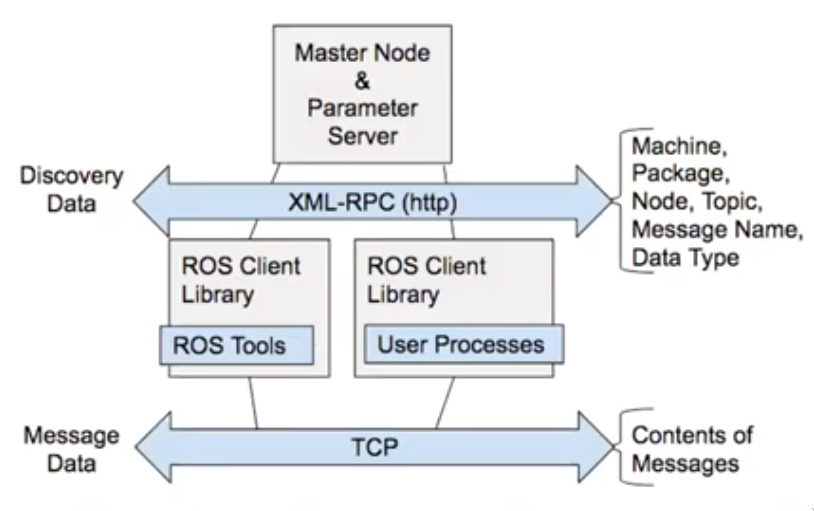
\includegraphics[width=0.5\linewidth]{images/former-ros1-architecture.png}
        \caption{Robot Operating System architecture.}
        \label{fig:ros1-architecture}
\end{figure}

The former communication architecture supported by ROS focused on a centralization perspective, as it had a implementation of a \textit{Master node}, that controlled every aspect of the communication establishment, meaning that every information exchange between nodes had to go through this master. A ROS Master node must be initialized before any node, as these nodes must also be able to address the ROS Master's location. The ROS Master was also in charge of the parameters, which offer important runtime information about the network nodes.

Due to the sheer wide capabilities controlled by the master, this centralization approach fits the purposes of a research tool, as it is simpler to monitor and analyse the system behaviour. This communication architecture, however, does not scale well since it is heavily reliant on the master node's availability, making it unsuitable for safety-critical and real-time applications. If the master fails, the entire system fails, representing a single point of failure and a huge performance bottleneck.

Many research communities tried to fix these real-time issues by proposing potential solutions, while supporting the same architecture design, that did not fully accomplished the needs of real-time applications. So, it became clear to the ROS community that the framework had architectural limitations that could not be rearranged using the same design approach. \cite{maruyama2016exploring}

Robot Operating System 2 comes as a complete refactoring of ROS, with the aim of increase the framework's real-time capabilities, by allowing the development of time-critical control over ROS, as it moves away from the former architectural design towards the implementation of an external middleware that can support the production needs of the outgrowing robotic systems. \cite{kim2018security, casini2019response}

%This lead to the creation of \textbf{ROS2}, which continues to provide a simple, uniform message passing interface to allow components to communicate with each other, now implemented using the Data Distribution Service (DDS) communication protocol as middleware. This means that there is no need to implement a master, making the system fully distributed. The discovery process between nodes is distributed and guaranteed by DDS, giving theses nodes the capacity to discover other nodes. Considering that there is no ROS Master implemented, the approach when dealing with the parameters also changed. Instead of having a global parameter server, in ROS2 each node declares and manages its own parameters. All these aspects related to ROS2 will be later discussed.

\subsection{Robot Operating System 2}

The Robot Operating System 2 (ROS2) was developed with the goal of easing the former ROS architecture. Although ROS2 continues to provide a simple, uniform message passing interface to allow components to communicate with each other, instead of implementing their own middleware specification, Data Distribution Service (DDS) communication protocol is implemented as an abstract middleware interface, through which serialization, transport and discovery is being provided. This implies that adding and integrating a new component into an existing system remains reasonably simple for a ROS developer.

\subsubsection{Data Distribution Service}

The Data Distributed System \cite{3}, simply known as DDS, is a Object Management Group (OMG) middleware standard, resulted from the need of better interoperability between different vendors middleware frameworks, directly addressing data communication between nodes that belong to a \textit{publish-subscribe} communication architecture, for real-time and embedded systems, that relies on a data-centric approach. DDS disposes a software API supported by a rich documentation about its exact behaviour. By furnishing this specification, it enables third parties applications, such as ROS, to implement this middleware, while auditing and understanding matters are covered by its documentation.
            
A middleware, such as DDS, is a software layer that sits between the Platform layer, which handles both the operating system as the network transport configuration, and the Application layer, that is usually implemented by sytems that highly rely on timing-measures and efficiency, when it comes to data-delivering between nodes. DDS aims to ease the complexity behind creating each sytem's own middleware, by handling relevant aspects like network configuration, communication establishment, data sharing and low-level details. As a result, system developers can mainly focus on their applications purposes, rather than concerning about information moving across levels. 

% Data centricity
The architecture approach is based on a concept named \textit{Data-Centric}, that instead of focusing on the reliable transmission of the message, the distributed infrastructure takes more responsibility, where the message-data itself is the focal point. Here, the infrastructure formally defines the data and imposes rules over it, with the continuous awareness of the contents in the data space, where known structures exchange these contents. Rather than forcing each application to deal with this complexity of defining the data space, DDS directly implements and provides controlled, managed, secure data sharing. However, the Data-Centric approach does not define the full DDS architecture, but only how messaging is treated.

DDS leverages the premise of a transport-independent virtualized Data Bus, to address the distribution of network resources, in which stateful data is distributed through the network, where multiple applications can acess this data in motion, representing an architecture with no single point of failure, respectively enabling a realiable way of ensuring data integratity. Consequently, by adopting this approach, the load on the network is independent of the number of applications, making it easily scalable. DDS communications are also governed with explicit \textit{Quality of Service} settings, that allows the system to manage and monitor which applications are able to communicate in which ways with the Data Bus and with each other. 

\begin{figure}[H]
    \centering
    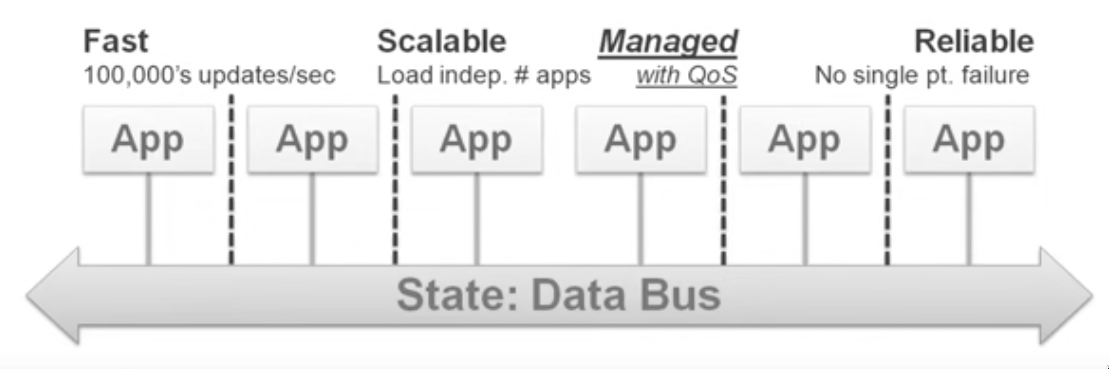
\includegraphics[width=0.6\linewidth]{images/dds-architecture.png}
    \caption{Data Distributed System architecture.}
    \label{fig:dds-architecture}
\end{figure}

When it comes to easing the communication establishment, DDS features a set of discovery services, allowing the automatic discovery between participants. As to adress the data transportation, DDS offers a wire specfication protocol called Real-Time Publish-Subscribe Wire Protocol (RTPS) \cite{rtps}, allowing multiple applications, that could differ on their used DDS implementations, to interoperate with each other as network domain participants, by abstracting and optimizing transport. 

Furthermore, RTPS was designed to make use of \textit{Quality of Service} profiles, where multiple transport policies can be specificed, that by default DDS does not support. For instance, as multiple DDS vendors are built over the UDP \cite{udp} transport protocol, which does not feature reliable delivery of data, transport reliability, often required by real-time environments, can be ensured by specifying the realiability corresponding QoS policy into the RTPS communication layer. Besides, QoS profiles also enable security deployment into the transport configuration. This approach offers flexibility over communication configuration and development versatility, allowing the developer to specify whatever QoS satisfies its system communication needs

A domain participant enables an application to participate in the global data space, either as a \textit{data writer} or as a \textit{data reader}, according to their role on how data, concerning their respective communications, is passed from point to point. Moreover, concerning the RTPS protocol, the communication architecture is based on a \textit{publish-subscribe} model. Each data writer publish data to a corresponding \textit{topic}, acting as a data \textit{publisher}. A \textit{topic} represents the data space objects through which data is handled. A data reader, complementing the role of the data writer in the RTPS data transportation, declares the intent to subscribe to the topic, in which data is published by the data writer, acting as a \textit{data subscriber}. 

\begin{figure}[H]
    \centering
    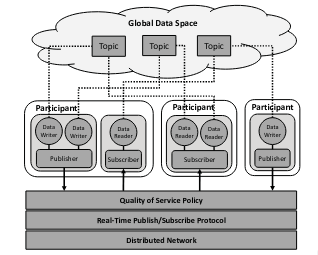
\includegraphics[width=0.5\linewidth]{images/dcps-model.png}
    \caption{Data Centric RTPS model. Extracted from \cite{maruyama2016exploring}.}
    \label{fig:dcps-model}
\end{figure}

Additionally, each domain entity manages the data according to the Quality of Service profiles speficified over the RTPS protocol, that is used over the transportation process as a policy. Applications within the network are then generated as DDS domain participants, with regard of the transport QoS policies. 

% Introduzir as implementações e DDS specifications

\subsubsection{DDS integration in ROS2}

As previously stated, the Robot Operating System 2 was developed to address the lack of support for real-time systems that the former ROS provided, mainly due to its architecture design that relied on their own middleware specification. To address this, ROS2 middleware approach is built upon the DDS framework \cite{maruyama2016exploring}, leveraging DDS for its messaging architecture, where communication and transport configuration are handled. As a result of the DDS integration, ROS2 applications are actually considered DDS applications, meaning that is possible to interoperate both native DDS applications and ROS applications, providing flexible compatibility.

By relying on an outside middleware, the modularity approach that ROS makes use of, where multiple modules should be applied when needed, while reducing the number of dependencies attached, highly depends on the middleware implementation that is being used. As far as dependencies are concerned, DDS implementations have light sized dependencies, often related to language implementation libraries, easing the complexity behind installing and running dependencies for ROS developers. \cite{ros-on-dds}

ROS2 middleware implements an interface on top of DDS, called \textit{ROS client library} (RCL), which hides much of the complexity of DDS specification API, offering a more friendly approach for the ROS users. However, it still provides access to the underlying DDS implementation for users that might want to integrate different DDS implementations for their use cases.

\begin{figure}[H]
    \centering
    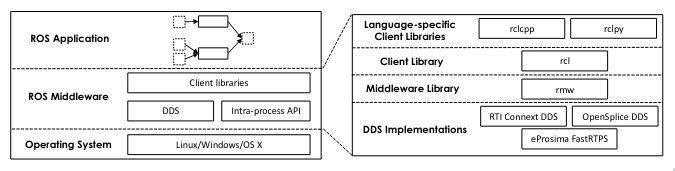
\includegraphics[width=0.5\linewidth]{images/ROS2-architecture.png}
    \caption{ROS2 framework architecture.}
    \label{fig:dcps-model}
\end{figure}

Towards supplying a wide range of configurations back to application layer, to vastly cover the robotic applications needs, ROS2 aims to support multiple DDS implementations, in which these implementation's API specification might differ from each other. In order to abstract from the specifics of these implementation's APIs, an abstract interface is being introduced, depicted above as Abstract DDS Layer, allowing portability among DDS vendores, which consequently enables ROS developers to interpolate DDS implementations, based on their application's needs during runtime. It should be noted that the DDS implementations are low-level of abstraction, strictly defined by its corresponding vendor's API. DDS only defines fundamental procedures at a higher degree of abstraction.  

% This layer could be removed, if there was no need to use more than one DDS implementation. But this is not the wanted scenario, since it is way more practical to switch the DDS implementation depending on the application needs. 

The former version of ROS already provided this abstract layer, customized and implemented by ROS client library, that allowed the communication between the Application Layer, in hwich the Master node was implemented, and the communication protocols. However, the capabilities offered by this middleware are significantly lower than ROS2 middleware, due to the DDS integration, as well as the fail to support the needs of multiple systems.

As stated, ROS client library hides the complexity of the DDS specification API from the developer. As RCL works under ROS structures, to keep the passing of information through the middleware layer, a structure mapping between ROS and DDS must occur. The data structure mapping between ROS and DDS must account the preservation of the former ROS messages' structure. The RCL works under the ROS messages' \texttt{.msg} files, and explained, these messages must be converted into messages' \texttt{.idl} files, to be used by the DDS transport.

The data transformation accounts the DDS implementation that is being considered at runtime, implemented at the \textit{Abstract DDS Layer}. The converted data is handled by the DDS wire protocol, RTPS, where the DDS publish-subscribe architecture and their respective structures comes to practice. Then, the reverse process must be ensured as well, to fully complete the information flow, where the data must be converted back to ROS structures before being returned to the ROS client library. \cite{ros-on-dds}


\subsubsection{ROS2 Graph Architecture}

As previous stated, ROS provides a way of data distribution between nodes base on published and subscribed data. Before considering about how the data is passed and treated by publishing and subscribing, nodes must be studiedly covered.
            
\textbf{Nodes} can be perceived as processes that will likely perform computation over the network. The network is comprised of many nodes, running simultaneously and exchanging data between them, with each node having its corresponding module purpose. Generally speaking, nodes are programs, built over a package, where their software code treats data that has been exchanged to each of them.

In ROS2, there is a modular convention about how to program nodes, where each class inherits from the Node object, easing the life of the programmer.        
For instance, lets considered a well-known example called \texttt{TurtleSim}, which is a simulator typically used for learning ROS, mainly composed by 2 nodes, that perform together towards moving a turtle. Additional nodes were implemented so security matters could be supported. After launching each node using the predefined ROS2 run command, \texttt{ros2 run <package\_name> <node\_name>}, the running nodes can be easily checked using the command \texttt{ros2 node list}. Note that, each node has its corresponding package, and nodes can be connected within a single package or between multiple packages.

\begin{figure}[H]
        \centering
         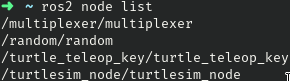
\includegraphics[width=0.4\linewidth]{images/ts_nodelist.png}
\end{figure}
    
The communication between nodes is done by message-passing, where the nodes involved exchange information through \textbf{messages}. A message is defined by its type, also known as its \textbf{interface}, which can be primitive (integer, string, boolean), or can be defined by a complex data structure, where multiple data types are assigned to their corresponding variables.

The message that triggers the turtle movement, in the \texttt{Turtlesim} example, is composed by multiple data movement variables regarding the linear and circular movement of the turtle. The interface is called \texttt{Twist} and it is a ROS predefined geometry message.

\begin{figure}[H]
        \centering
         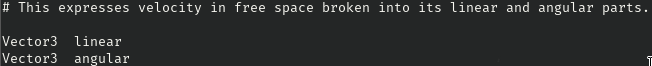
\includegraphics[width=0.7\linewidth]{images/ts_interface_twist.png}
\end{figure}
            
Messages are passed through via the pattern of publishing and subscribing over a \textbf{topic}. A node publishes the message to any number of topics, that are then subscribed by nodes that want to get access to that message. Topics provide a multicast routing scheme, where publish data can be casted into multiple subscribers.

\begin{figure}[H]
        \centering
        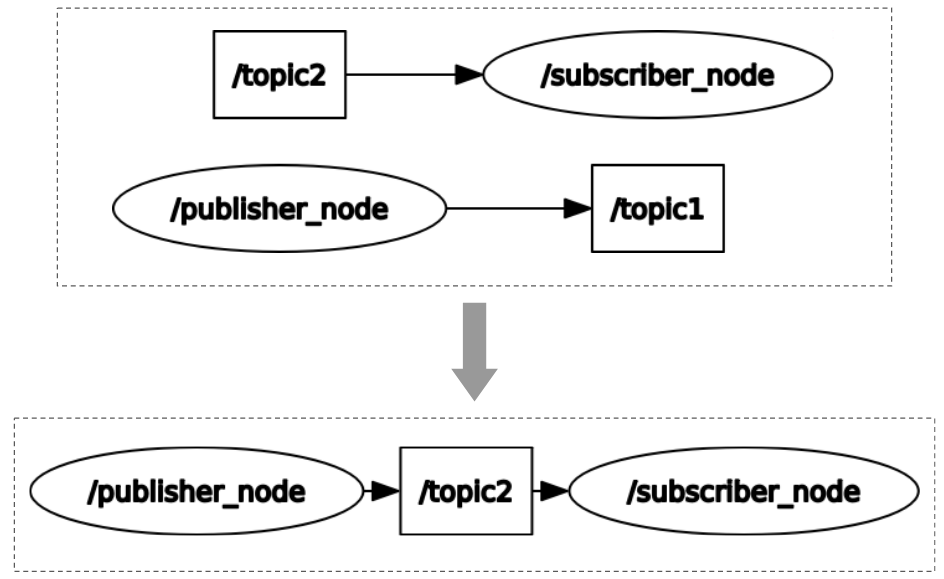
\includegraphics[width=0.7\linewidth]{images/ros2-topics.png}
\end{figure}
            
The topic is created upon specifying in the node either a publisher or a subscriber instance, providing the topic name as an argument. After building and executing the node, their associated topics are created. The available topics can be listed by running the predefined ROS command \texttt{ros2 topic list}.
            
\begin{figure}[H]
        \centering
         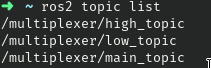
\includegraphics[width=0.3\linewidth]{images/ts_topiclist.png}
\end{figure}
            
If the nodes that want to exchange data through a topic are implemented in the same package, the respective subscriber and publisher nodes must have the same topic name instantiated. The configuration is pretty simple, whereas if the nodes are specified in different packages, a technique of \textbf{remapping} must be used.

The topic list related to the \texttt{Turtlesim} is depicted above. The 3 listed topics are vital for the communication process, and they all correspond to the \texttt{multiplexer} node. This happens because remapping between topic names is used to establish communication between packages, as explained above.

Both launching and remapping process are done by running a ROS \textbf{launch file}, that simultaneously launches each node, providing a simpler way of monitoring the system nodes. 

\begin{figure}[H]
        \centering
         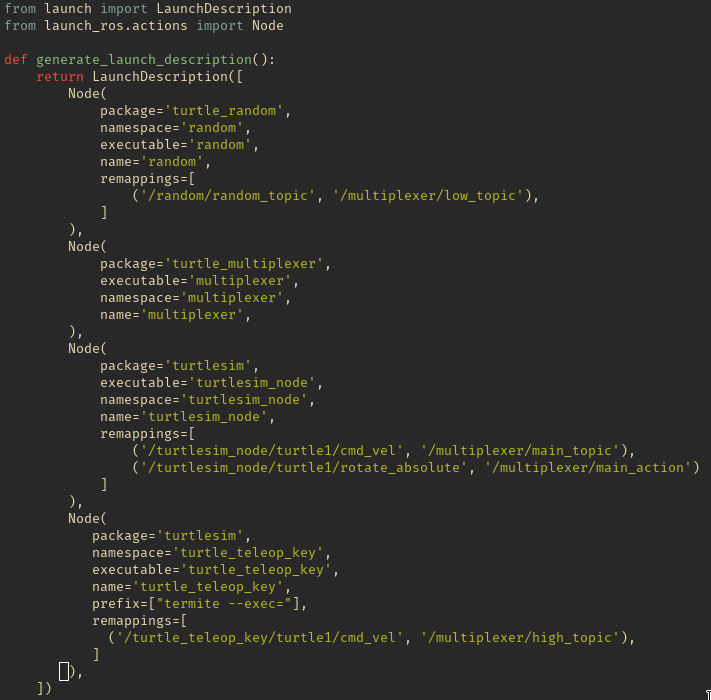
\includegraphics[width=0.3\linewidth]{images/ts_launch_file.png}
\end{figure}

As it can be seen, every node is instantiated in this file, and have each topic remapping defined in \texttt{remappings} section. Also, distinctive namespaces allow the system to start the nodes, without any name nor topic name conflicts. However this technique has some flaws attached, since it does not furnish a way of launching nodes in a separated terminal, needed for user interaction purposes, like input reading.

Running the following ROS command \texttt{ros2 launch <file\_name>}, will automatically compile and run the launch file.

\begin{figure}[H]
        \centering
         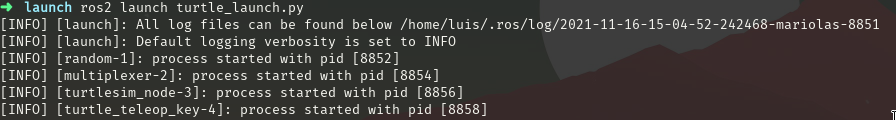
\includegraphics[width=0.7\linewidth]{images/ts_launch_ros.png}
\end{figure}

Every network node is now running simultaneously in the background. The only foreground running node is the turtlesim one, because it has an associated interface showing the turtle movement.

\begin{figure}[H]
        \centering
        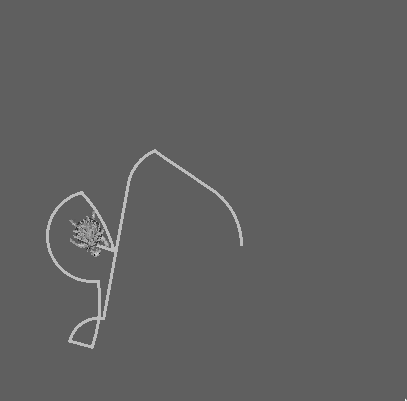
\includegraphics[width=0.3\linewidth]{images/ts_turtle.png}
\end{figure}

For understanding reasons, the reader may want to see how does the network architecture is organized. ROS2 provides a GUI tool called \textbf{rqt}, that helps the programmer in manipulating the network elements, in a more user-friendly way. This tool has a graph visualizer plugin that allows the programmer to view the network graph and how the elements are connected.

While the nodes are running in the background, the reader may want to run the following command \texttt{rqt\_graph}, in a separated terminal. The network graph related to the \texttt{TurtleSim} is represented bellow.

\begin{figure}[H]
        \centering
         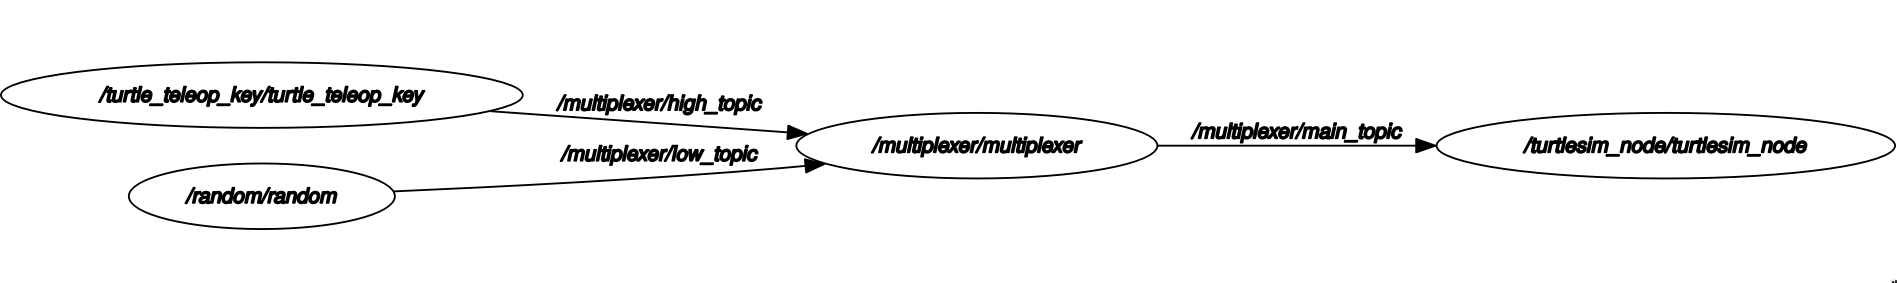
\includegraphics[width=\linewidth]{images/ts_rqt_graph.png}
\end{figure}

The \texttt{multiplexer} node, being the main node in this particular network, subscribes to two different topics from two different nodes.

--- The \texttt{turtle\_teleop\_key} node corresponds to a keyboard controller, that sends movement commands through the \texttt{high\_topic} to the \texttt{multiplexer}.\\
--- The \texttt{random} node sends random movement commands through the \texttt{low\_topic} to the multiplexer.

Since the \texttt{multiplexer} has two different active subscriptions, managing two different turtle movement values, it must keep them synchronized with each other. This is achieved by setting different priorities to each subscription, where the keyboard node has priority over the random controller, meaning that when the keyboard publishes movement data through its corresponding topic, the \texttt{multiplexer} must process that received data. \textbf{Timers} are also used, since they provide a useful way of managing these topics, by time-assigning, alternately changing the priority after the timer runs out, through its corresponding callback function.

The \texttt{multiplexer} also has a publisher instance defined, since it has an active connection through the \texttt{main\_topic} connection to the \texttt{turtlesim\_node} node, that is responsible for controlling and projecting the turtle movement. The \texttt{main\_topic} will be in charge of the values passed to the turtlesim node, instructing the turtle to move.

Given the priority set at each moment, the \texttt{multiplexer} has to forward the movement command, either from the keyboard or the random controller, through the \texttt{main\_topic}, enabling the turtle movement. Every aspect related to the publisher-subscriber pattern, in this ROS2 system, is treated over remapping of topic names. The data passed through the \texttt{main\_topic} can be checked using the command \texttt{ros2 topic echo main\_topic}. As expected, the data has both linear and angular vectors defined because of interface used.

\begin{figure}[H]
        \centering
        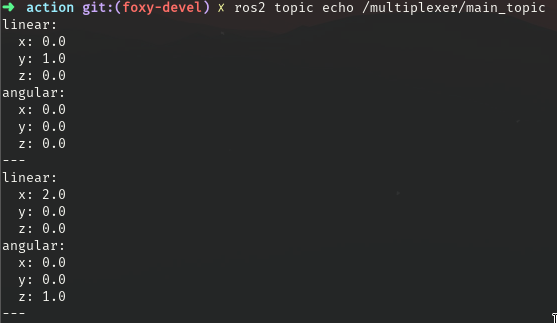
\includegraphics[width=0.5\linewidth]{images/ts_main_topicinfo.png}
\end{figure}

\subsubsection{Other ROS concepts}

The \texttt{TurtleSim} application given as example above, so the reader could get familiar with the basics concepts about ROS, does not address all the existing ways of data-exchanging between nodes.
                
Even though topics are the most conventional way of communication, because of its multicast scheme, subscribers can not be perceived by the publishers, so logging and matching becomes rather difficult. Node synchronization within the network is also not featured by topics.

\paragraph{Services}

\textbf{Services} allows a client, that can also be seen as a topic subscriber, to request data from a server, that likewise a topic publisher, furnish data through a service. Services works under a synchronous policy, since the data is only provided when the client node makes a request. Each service is always linked to just one server node, and does not maintain active connections.
                
In ROS1, services used to work under a synchronous policy, where the service client would stall waiting for the response of the service server. While, in ROS2, services are \textbf{asynchronous}, since it is possible to specify a callback function that is triggered when the service server responds back to the client.

\begin{figure}[H]
    \centering
    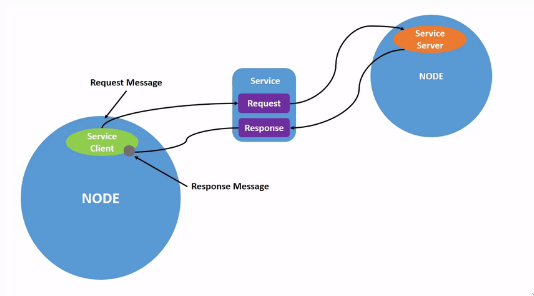
\includegraphics[width=0.7\linewidth]{images/ros2-services.png}
\end{figure}
                
                
The interface used on services messages differ from the topics interface. That is because a service is composed by a request and response, so their data structures may differ. 

Suppose, considering the \texttt{TurtleSim} example, that a client wants to make a request to move the turtle by providing coordinates (valued in integers) and a \textit{theta} angle. A conventional way of the node server sending a response back to the client is by passing a boolean value, ensuring that the request has been processed, and a string value regarding the name of the turtle. By that, it must be considered two different data structures. Therefore, this considered service interface should be similar to the following:

\begin{verbatim}
    float32 x
    float32 y
    float32 theta
    ---
    bool check
    string name
\end{verbatim}

\paragraph{Actions}

Another way of exchanging data is by setting goals through \textbf{Actions}. Actions, likewise services, also uses a client-server model, but they were design for other purposes rather than only processing a request and sending back a response. Actions are intended to process long-running tasks, where the client sends a goal request to the server node, that confirms the receiving of this goal. Before returning a response back to the client, the server can send feedback back to the client. Unlike services, actions can be cancelled, so the return response could not be acknowledge. 

\begin{figure}[H]
    \centering
    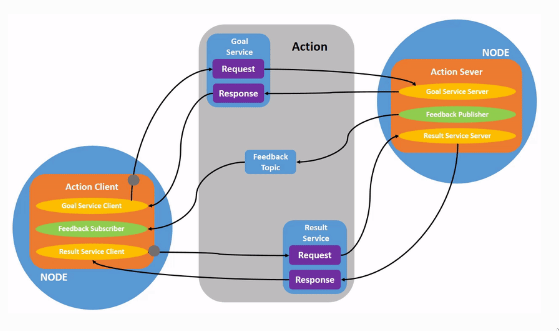
\includegraphics[width=0.7\linewidth]{images/ros2-actions.png}
\end{figure}

The interface structure used in actions is also different from the others, since it provides an additional data structure to the services interface, corresponding to the feedback feature that actions provide.
                
Considering the same example of the \texttt{TurtleSim}, a client may want to request a goal providing a \textit{theta} angle, to trigger the turtle rotation. To keep the client updated, one way of the server feedbacks the client is by sending the angle rotation that is left to be executed. After the execution, the server may want to acknowledge the client by confirming the angle passed as a request, confirming that the rotation has been executed properly. By that, it must be considered three different data structures. Therefore, this considered service interface should be similar to the following:

\begin{verbatim}
float32 theta
---
float32 delta
---
float32 remaining
\end{verbatim}

This given example is commonly used in robotic systems for navigation, where the robot travels to a position, previously requested by a client. While its traveling, it can send information about the transition state. When the robot reaches the predefined position, the server acknowledges the client by sending a result message. 

Note that, in both interfaces introduced, the \texttt{---} divides the each structure that are used in each communication. In services, the request structure must be separated from the response structure. In actions, there is also the feedback structure which is the last structure defined.  
               
\paragraph{Parameters}
               
Another relevant concept behind ROS is the existence of nodes \textbf{Parameters}, that allows individual configuration of the network nodes. In the former version of ROS, the node parameters were controlled by a shared \textbf{Parameter Server}, managed by each ROS Master node responsible for the its corresponding network. As stated before, in ROS2 each node declares and manages its own parameters. Usually parameters are saved using files related to the nodes, but parameters can also be updated and checked using \texttt{get} and \texttt{set}, respectively. Additionally, using a parameter function callback, the node's parameters can easily be edited.
               
\paragraph{Interfaces}
               
Although it was already mentioned, since it was needed for explaining each method of communication for nodes in ROS, \textbf{Interfaces} should be duly studied.
As explained before, each type of communication has its different corresponding interface, and they must be specified in different folders with unique namespaces.
The folder namespaces used are the following:
\begin{itemize}
    \item[---]Topics messages: \texttt{msg/}
    \item[---]Services messages: \texttt{srv/}
    \item[---]Actions messages: \texttt{action/}
\end{itemize}
               
Recall the \texttt{TurtleSim} example and its corresponding package \texttt{turtlesim}. Suppose a case where, it could be possible to add boxes into the turtle GUI, blocking the turtle movement though those boxes. To add boxes, the topic message considered should have two different values regarding the $x$ and $y$ axis value related to the turtle map. This interface could be named as \texttt{Boxes}, with the \texttt{.msg} extension (\texttt{Boxes.msg}).
               
\begin{verbatim}
    float32 x
    float32 y
\end{verbatim}

In your node's code, the following import must be specified:

\begin{verbatim}
    turtlesim/msg/Boxes
\end{verbatim}
               
\paragraph{Lifecycled Node}
               
ROS2 introduces a new definition of node, called \textbf{lifecycled node}, as addition to the traditional one. A lifecycled node is defined by its current state. Its state can either be unconfigured, inactive, active or finalized. This can be useful, since it provides a structural way of setting up the node and separating all its state functionalities. The transition through states are done by running a callback function. Nodes that need initial configuration before exchanging data within the network can be perceived as lifecycled nodes, like sensors, where its detection must be ensured before the data reading/publishing process. 
               
\paragraph{Node Composition}
               
A concept that both ROS and ROS2 provides is the idea of composing nodes into a single \textbf{process} for improved \textbf{performance}. Usually a node is attached to a single process, but it is possible to combine multiple nodes into a single porcess, structurally abstracting some network parts. 

There is a slight difference about how ROS and ROS2 approaches the node composition. In the former version of ROS, node composition was done over the combination of \texttt{nodelets}. In ROS2, instead of calling it a \texttt{nodelet}, it is called a \texttt{Component}. 

Formerly, \texttt{nodelets} were designed to ease the cost of overusing TCP for message-passing between nodes, that if the message consisted huge sized data could negatively affect the performance on the network communications. By grouping performance critical nodes, nodelets provided a local way of message-passing between the considered nodes.

Supported by the former idea of \texttt{nodelets}, \texttt{components} are compiled into shared libraries. A component itself does not furnish node composition, since a component is a node with special features. Although,  each component can be loaded into a \textbf{component container} process at runtime in the network. By loading components into these containers, the node composition is ensured. 
 
Note that, nodes do not provide this feature since they are compiled into executables that need to be previously compiled. Components can be also be configured to be loaded at compile-time, where a single executable runs multiple components. Components can be also configured in a ROS launch file, using containers as well.
 
Node composition could also be applied for security matters. Suppose a scenario where multiple nodes respect the same security policies. By combining them into a single process, the mapping into this set of rules would be direct, easing the usage of security enclaves. % Although, this idea seemed promising, it caused non-negligible overhead due to composition of nodes, so ROS2 introduced a new mapping approach. 
This is will be later explained in the \texttt{security} section.
% Node composition can be also useful for security matters, since it can ease the creation of \textbf{security enclaves}. An enclave is a set of nodes that follow the same set of policy rules. This is will be later explained in the \texttt{security} section. 
               

\subsection{The need for Security}
        
A major factor behind its popularity and widespread adoption is its flexibility and interoperability. In ROS, this flexibility was valued above all else, meaning that values like security were not considered as a priority, so ROS applications tend to face increased security risks. 
            
Also, ROS works over a publish-subscribe pattern, which is very useful, since it brings various forms of decoupling and transparency. However, because of this transparency, publishers within ROS are unable to control the consumption of their data and subscribers, most of the times, cannot identify the integrity of their received data. % The low barrier to entry and open nature of the ROS ecosystem % 
This means a malicious actor could potentially inject code or vulnerabilities into a library, which could then be reused by another unsuspecting developer.

These concerns about security take on particular importance, since robots are becoming more frequently used and can directly affect the physical world. \textbf{Cyber-physical} systems, commonly related to the arising of the automatizing concept of robots, feature unique vulnerabilities that exploit both cyber and physical nature of these devices, mainly by sensing and actuating. Sensing becomes relevant when it comes to the potential leak of information about the surroundings of its robot. Whereas, actuating is related to the functionality of the robot, where physical safety is the main concern.\cite{8794451, mcclean2013preliminary} % One of the most interesting results of the honeypot experiment is that it can be very difficult to discern between a cyber-physical  security  exploit  and  hardware  and/or  software  bugs. %

ROS faces known vulnerabilities due to its architecture and model nature. ROS internal communication is built around TCP ports, allowing robots to be built using several modules, that can be distributed. However, this modularity results in the exposure of TCP ports, that usually leads to attacks that compromise the data itself.
There is also a concern about how ROS manages the communication between nodes. In ROS, the node-to-node communications are settled in plain text. Despite the fact that this way of handling communications bring certain benefits, especially better performance and data recovery, it is evident that data content is vulnerable to unauthorized usage.

As discussed previously, this is mainly due to the fact that ROS had its own middleware, which didn't provide any security features. The 'centralization' behind ROS architecture, where everything was controlled and connected to the ROS Master node, was also a major fact to the need of a new implementation where the middleware could not also facilitate the establishment of communications, but also could provide security features. ROS2 adoption of middleware interface for data exchange offers a flexible way to build appropriate defenses for a given application.

DDS ensures not also communication features, but also guarantees security properties, where ROS's flexibility is preserved despite this increase on security. The \textbf{DDS-Security} is a specification that serves as an add-on to the DDS specification, defined by a set of plugins combined in a Service Plugin Interface (SPI) architecture. The main plugins provided by DDS-Security are the following ones:
            
\begin{itemize}
    \item[---] \textbf{Authentication}: Verification of each identity of a given Domain Participant, by assigning a private key and a public key to each one, as well as an certificate that relates the participant's public key to its corresponding specific name.
    \item[---] \textbf{Access control}: Provides control over DDS-related operations with the support of the Authentication plugin. It requires two files per domain participant signed by a Certificated Authority, that specifies how the domain should be secured and their permissions.
    \item[---] \textbf{Cryptographic}: Operations related to cryptographic purposes, such as encryption are handled by this plugin.
    \item[---] \textbf{Logging}: Provides logging over events.
    \item[---] \textbf{Data tagging}: Add tags to data samples.
\end{itemize}

\begin{figure}[H]
    \centering
    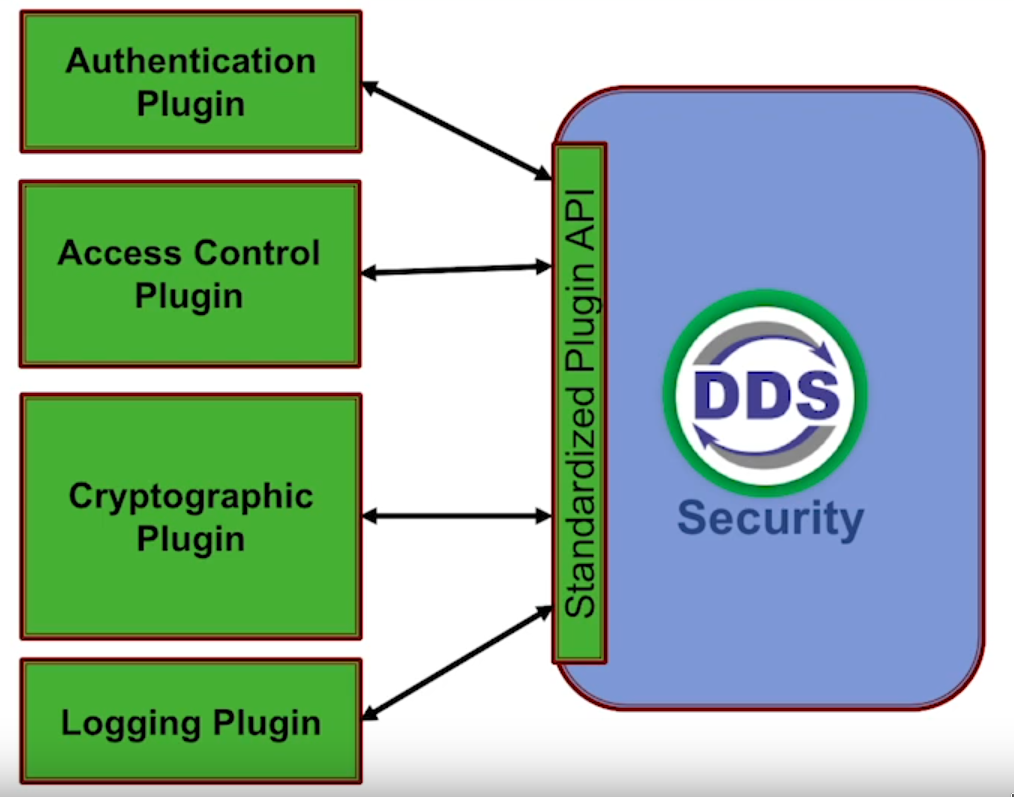
\includegraphics[width=0.5\linewidth]{images/dds-security.png}
\end{figure}
            
These plugins can be customized since different applications require different needs when it comes to security. That is why, as depicted above, there must be a \textbf{Standardized Plugin API} that acts as an interface between modules and DDS security protocols, while including all aspects of secure communications. 
ROS2 is deployed without security mechanisms by default, but DDS can provide security guarantees such as authentication and access control with a variant called DDS-Security. Using DDS-Security it is possible to configure ROS2 to run with security guarantees using the \textbf{SROS2} toolset. Most of these tools supported by SROS2 is contained within the ROS Client Library (RCL), and includes the following features:

\begin{itemize}
    \item[---] Support for security files for each domain participant, where in ROS2 are seen as a process, and each process must be associated with a set of these files.
    \item[---] Support for both permissive and strict enforcement of security, meaning that can be considered two approaches when it comes to dealing with security files.
    \item[---] Support for a master “on/off” switch, that enables or disables every security feature.
\end{itemize}

The SROS2 has been designed to work with any secure middleware. However, not all middleware is considered open-source and highly depends on the ROS distribution in use.

Since this security process involves a lot of new technology, the user must be aware of improper configuration, that can still lead to security problems. However, SROS2 CLI include a tool, named \texttt{ros2 security}, that aims to help those who don’t want to set it all up by themselves.

\subsubsection{TurtleSim with SROS2}
            
Now that the concept behind SROS2 is introduced, the \texttt{TurtleSim} application given as an example in the previous section, can now  be treated using security features related to the nodes involved.

The \texttt{multiplexer} node handled the commands responsible for the turtle movement. Note that, the turtle is implemented in the \texttt{turtlesim} node, so both \texttt{multiplexer} and \texttt{turtlesim} nodes are directly connected through a specified topic. \texttt{Multiplexer} acts as topic selector between two different subscribed topics, where each of them was respectively associated with a priority. Based on the priority set at each moment, the \texttt{multiplexer} node forwards the command related to the selected topic into the \texttt{turtlesim} node, by topic remapping, which triggers the turtle movement. Even though the \texttt{multiplexer} handles the two specified subscribed topics that receive movement data from both \texttt{random controller} and \texttt{keyboard} nodes, its not exclusive to the \texttt{turtlesim} node, as it is still possible to directly publish commands to the topic that handles the turtle movement, since the security properties have not been implemented yet.

In order to guarantee this exclusivity where the \texttt{multiplexer} is the only node that directly publishes data to the topic that enables the turtle movement, is by specifying \textbf{access control} files. The remaining nodes should be considered as untrustworthy, denying any potential undesired turtle movement originated by these nodes that tried to publish data through the topic. The idea is to encapsulate both \texttt{multiplexer} and \texttt{turtlesim} nodes, as the \texttt{multiplexer} monitors and manages all the data intended to manipulate the turtle movement, similar to a reversed proxy server.

\begin{figure}[H]
    \centering
    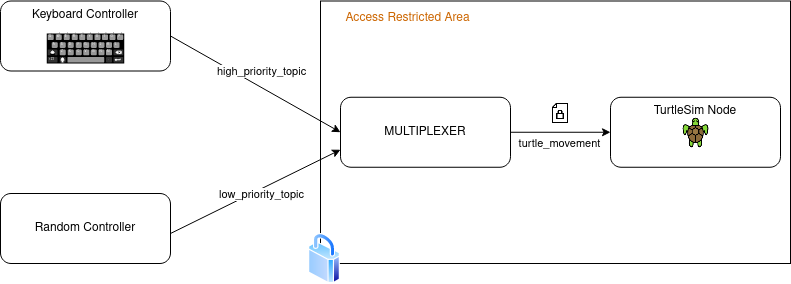
\includegraphics[width=0.8\linewidth]{images/ts_secured_multiplexer.png}
\end{figure}

Note that, as it is now, the only nodes that are supervised by the \texttt{multiplexer} are the \texttt{random controller} node and the \texttt{keyboard} node. However, it can be implemented new nodes with ease, as it is only required to remap topics in the launch file and create as many subscriptions in the \texttt{multiplexer} as many implemented nodes.

So, in technically terms, a \textbf{SROS2 keystore} must be initiated. ROS2 provides a command that permits the creation of \textbf{keystores} by using the \texttt{security} keyword. This command enables features regarding security matters, that has access to the SROS2 tools related to the DDS-security artifacts.

The keystore is a created directory where DDS security features are stored. By creating a keystore directory, then it can be later sourced to be used by RCL to provide security to the associated ROS2 network.
            
\begin{verbatim}
    ros2 security create_keystore turtlesim_keystore
\end{verbatim}

The created keystore directory structure is displayed bellow:

\begin{figure}[H]
    \centering
    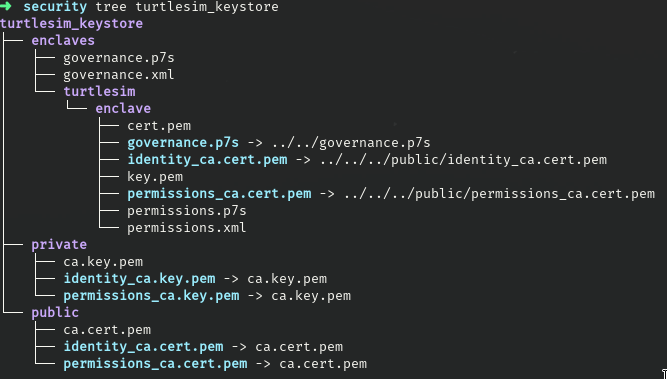
\includegraphics[width=0.6\linewidth]{images/ts_keystore_tree.png}
\end{figure}

By creating the keystore, three different sub-directories will be generated.

\begin{itemize}
    \item[--] The \texttt{enclaves} directory contains the security tools related to each enclave created. An \textbf{enclave} is a group of ROS nodes, controlled by the same set of security rules, defined in its corresponding enclave directory. Each enclave includes files needed to enable security, such as CA certificates and their own private key (\texttt{key.pem}). Besides containing each enclave created (for instance, in the figure above, a \texttt{/turtlesim/enclave} enclave is created), this directory also has a governance policy document \texttt{governance.xml}, as well as a signed copy file related to the CA permissions, \texttt{governance.p7s}. 
    \item[--] The \texttt{public} directory contains material that is permissible as public. A Certificate Authority certificate, \texttt{ca.cert.pem} is stored in this directory. This file stores the CA \textbf{public key} and it is used to validate the identity and permissions of each ROS network node by the CA. Note the existence of \texttt{identity} and \texttt{permissions} folders with their respective certificate/key file. This is due to the fact that DDS supports the separation of identity and permission chains, however ROS usually uses the former \texttt{ca.cert.perm} file, meaning that only a CA is used for both these processes.
    \item[--] The \texttt{private} directory contains material that is considered private. A Certificate Authority certificate, \texttt{ca.cert.pem} is stored in this directory. This file stores the CA \textbf{private key}. It is used to modify the network policies, such as access permissions, and to add new participants. Similar to the \texttt{public} directory, the CA key corresponding to its identity and permissions can be stored in their corresponding individual directories.
\end{itemize}
            
The reader may want to create as many keystores as needed, but RCL can only use a keystore's artifacts at once. The directory is defined by the SROS2 environment variable \texttt{ROS\_SECURITY\_KEYSTORE}, that needs to be previously sourced. Environment variables sourcing will be explained further on.

Once the keystore has been created, the respective enclaves can be implemented. By using the tag \texttt{create\_key}, with the keystore namespace provided (in this case is \texttt{turtlesim\_keystore}), each enclave can be created.

Although the idea of enclave has already been introduced, the full context behind it is yet to be explained. As mentioned, an enclave is a group of ROS nodes that follow the same security policy. Since an enclave is a DDS domain term, typically a node is an abstraction of a DDS \texttt{Participant} (previously mentioned as a Domain Participant). In ROS2, the usage of an enclave is done upon running a node, which causes the creation of a running process. This means that, enclaves are used by processes, providing them security based on their artifacts and specification. 

Since the mapping is between processes and enclaves, the reader may wonder, if node composition into a single process is a reliable way for matching multiple nodes simultaneously to the same enclave. Well, this is actually a good approach but nodes can not be perceived as domain participants, while considering node composition, due to the fact that composing participants results in non-negligible overhead. 

There is also not convenient to compose nodes as individual participants, as far as security is concerned. That is because each participant has its own security identity related to its node, and by composing participants, they all share the same OS memory space, consequently access data is shared between them, and permission distribution becomes rather difficult to handle. 

So, each participant must be matched to a node shared context, instead of being directly related to a specific node. 
            
% Note that, it is possible to combine multiple node contexts into a single process, meaning that multiple enclaves can be structurally contained in a single enclave directory (enclave hierarchy).

Each enclave security artifacts are used by each participant, meaning that each node mapped into the same context is controlled by the same enclave. 
%The mapping is between a participant and its corresponding set of security rules. However, the set of security rules can be also used by others participants, meaning that, in ROS terms, multiple nodes can share the same security context. 
Thereby, the initial given definition of an enclave is not totally correct, since a participant can either be perceived as single node or as multiple node shared context. 

Usually the node \textbf{namespace} are quite relevant upon creating enclaves, since the default way of implementing enclaves creates a namespace hierarchy path depending on the node namespace, so node remapping could affect its corresponding enclave path. With the introduction of node contexts, the enclave path is now disassociated from node namespaces, having its own resource identifier. This approach is also appropriate when composing nodes from different packages (that consequently have different namespaces) scenario is considered, where the path of the shared enclave must be common to each node. 
% The \textbf{Access Restricted Area} can not be implemented as illustrated above, since each key stored into the keystore previously initiated, is directly related to two different packages. So two different keys must be created, one for the \texttt{multiplexer} and other for the \texttt{turtlesim} node.

\begin{verbatim}
    ros2 security create_key turtlesim_keystore /security_enclave/
\end{verbatim}
            
In order to run these nodes concerning the created keys, all the packages related to the network must be re-built using the \textbf{Fast DDS} additional flag.
            
\begin{verbatim}
    colcon build --symlink-install --cmake-args -DSECURITY=ON
\end{verbatim}
            
The following exports need to be sourced to force SROS2 security features. The reader may want to put these exports into a shell script, and then add this to the \texttt{PATH} environment variable.
            
\begin{verbatim}
    export ROS_SECURITY_KEYSTORE=/path/to/the/created/keystore
    export ROS_SECURITY_ENABLE=true
    export ROS_SECURITY_STRATEGY=Enforce
\end{verbatim}

These exports are related to relevant SROS2 environment variables, that the reader must be aware when considering the SROS2 tools.

\begin{itemize}
    \item \textbf{ROS\_SECURITY\_KEYSTORE}: This variable sources the root of the created keystore. By sourcing this location, ROS2 knows where the security artifacts are stored.
    \item \textbf{ROS\_SECURITY\_ENABLE}: This variable is the SROS2 enabler.
    \item \textbf{ROS\_SECURITY\_STRATEGY}: As stated before, SROS2 provides two different approaches when it comes to dealing with security files. This variable handles that property, and it can be set either to \texttt{Enforce} or \texttt{Permissive}.
\end{itemize}

Now that all ROS2 security prerequisites have been successfully configured, the network can be launched. 

Since SROS2 has no support for launch files, each node needs to be launched separately on its own terminal, with regard of their respective keys. 
Later, this process is simplified by launching a shell script. 
            
\begin{verbatim}
    ros2 run turtle_multiplexer multiplexer --ros-args --enclave /multiplexer/multiplexer
                
    ros2 run turtlesim turtlesim_node --ros-args --enclave /turtlesim_node/turtlesim_node 
\end{verbatim}

As pointed previously, DDS has several implementations that can be considered when the ROS2 network is being configured. The ROS2 distribution usually dictates what is the default middleware implementation of DDS being used. Most of these ROS2 distributions uses the same default middleware implementation, which has the name of \textbf{Fast DDS} (formerly named \texttt{Fast RTPS}). The features that stand-out the most in this implementation are the promotion of an interface generator (\texttt{Fast DDS-Gen}) and the usage of \texttt{RTPS} communication protocol, which guarantees performance, real-time behaviour, efficiency, scalability and, most importantly, security. As explained earlier, the Fast DDS security flag, \texttt{-DSECURITY=ON}, must be considered upon building the ROS2 packages. Although, the reader may want to set a different DDS implementation. In order to do this, the reader should install the DDS middleware software, following the implementation specification and dependencies, and then rebuild the workspace forcing the DDS implementation to change. ROS2 has a environment variable, \texttt{RMW\_IMPLEMENTATION}, that allows the replacement of the middleware that is being used.

The creation of these keys only ensures that the communication between the \texttt{multiplexer} and the \texttt{turtlesim} is authenticated, and the exchanged data is encrypted, so Access Control is yet to be implemented.

By using tools like \texttt{tcpdump}, the data packets can be displayed and this encryption can be easily verified. If no SROS2 security is regarded (no export made), the data is passed in plain-text, as expected. After sourcing the security features, using the exports specified above, the packet displayed is encrypted, and its larger since additional information is considered to increase safety. % An encrypted packet example is illustrated in the following figure.  


\subsubsection{SROS2 - Automatic key generation}
            
Before considering applying access control to the \texttt{TurtleSim} example, let this SROS2 feature be introduced. SROS2 supplies tools to automate the process of generating enclaves and their respective permissions files. 

First a \texttt{policy.xml} needs to be created, while the ROS2 network is running with SROS2 security enabled, so that the file stores information about the network. 
                
\begin{verbatim}
    ros2 security generate_policy policy.xml
\end{verbatim}

Now, the created policy file can be used as a reference to automate the process of key generation. To do this, both keystore and policy must be given as arguments to the following SROS2 command.

\begin{verbatim}
    ros2 security generate_artifacts -k turtlesim_keystore -p policy.xml
\end{verbatim}

\subsubsection{Access Control}
            
In order to provide access control, the permission files, of the enclave that is being considered, need to be modified. This is ensured by adding security permissions to these files, with the mandatory signature of the CA. 
                
However, a suitable way of editing the permission file, \texttt{permissions.xml}, that dictates how the enclave manages the permissions within the network, is by creating a policy file and running the following command.
                
\begin{verbatim}
    ros2 security create_permission turtlesim_keystore /enclave policy.xml
\end{verbatim}
    
Besides changing the permissions file, the CA signature is also generated, meaning that the permissions modification have been successfully implemented in the considered enclave.

This \texttt{policy.xml} passed as an input for easing the alteration of the enclave permissions, follows a restrict SROS2 \textbf{policy XML schema}. This schema makes use of a few concepts, that are relevant to understand how the schema design was conceived.

\begin{itemize}
    \item[--] \textbf{Mandatory Access Control}: Permissions to allow the access to an object are pre-established by a set of authorization rules, and can not be modified by any subject.  
    \item[--] \textbf{Principle of Least Privilege}: This principle is to guarantee that only the minimum access privileges are used to the intended purpose.
    \item[--] \textbf{Privilege Separation}: The access privileges that a subject owns are separated, decreasing the possibility of a security vulnerability.
    \item[--] \textbf{Separation of Concerns}: Distribution of the system security concerns into each corresponding section.  
\end{itemize}
                
                % (short)
                % Relevant tags
                % Problems
                
                % What is intended in our example
                % How is it implemented
                % Policy file example


\section{Related work}\label{s:ros-relWork}

This section aims to present previous works that attended security matters related to the deployment of robotic systems using Robot Operating System as its application enhancer. When developing real-time systems, safety matters are often referred as critical, because of the overall integration with the real world. Security however, it is measured by evaluating different security issues by properly analysing the system model. However, due to the high nonlinearity and complexity of real-time systems, implementing such a thorough analysis method in near real-time remains a significant difficulty.\cite{diao2009design}

The deployment of real-time systems results in the importance of concerning about safety in a performance point of view, resulting of the demanding time-critical scenarios. Many studies were made regarding the performance in both ROS and ROS2 (also regarding DDS Quality of Service policies \cite{maruyama2016exploring}), by analysing using performance measurement approaches, providing a guided and supported review on how performance can directly affect time critical situations, where safety is envolved.\cite{maruyama2016exploring, casini2019response} 

System security concerning network exposure, often explored by unauthorized acess and data leaking, can be treacherous and it is considered a complex subject, due to the abundance of different network security technologies that do not cover every security aspect, since absolute security does not exist, as new vulnerabilites arise from the tecnology evolution.\cite{kaeo2004designing} The creation and deployment of security countermeasures are essential upon configurating the network towards achieving security. Within this vast topic, several different avenues of endeavor come to mind, each deserving of a substantial study. Network security means exploring the network beforehand by computer intrusion detection, traffic analysis, network monitoring, alongside many other practical networking security aspects.\cite{marin2005network}

The literature concerning the network security enhancment that Robot Operating System 2 furnishes, by offering the SROS2 toolset, is quite limited. Most of the existing work is on the exploration of the former version of ROS in terms of port exposure, contextualized in the approach considered to protect the system network.  

Many researches were made regarding this issue that ROS faces, one in particular that explored the IPv4 address space of the Internet for instances of ROS, named \textit{Scanning the Internet for ROS: A View of Security in Robotics Research}\cite{8794451}, with the goal of identifying ROS vulnerable hosts, mostly master nodes since they provide information about their related topics and node's parameters, mainly by port scanning, so that developers could be aware of the possibility of exposure of their robots. The performed scans furnished information about hosts that could either be a sensor, an actuator or even a simulator. Topics were also identified since they provide evidence of what is likely to be available to an attacker. This study is rather relevant because of how easily can attackers gather information about potential robots, and control them further on, through the public Internet, making it unavoidable to develop mechanisms concerning security.

A different approach was previously presented\cite{application-security-ros} when it comes to protecting the ROS network, which primarily focused on applying security measures on the application layer, treating ROS architecture as a black-box, by mainly running an Authentication Server, storing certificates and files related to trusted domain participants, while controlling and providing session keys related to the communication process. Even though the message data can not be perceived, unauthorized nodes can still collect information about the flow of the data, since ROS architecture is responsible for the publish-subscribe interaction, meaning that security issues still persist which cannot be handled on the application level alone.  

Secure Robot Operating System (SROS)\cite{white2016sros} was initially developed as an experimental tool (later evolved to SROS2 as a supporting tool for ROS2), which supports TLS for all socket transport, node restrictions and chains of trust, guaranteeing publishers authorization when it comes to publish to a specific topic. Another worth-mentioned tool is Rosbridge\cite{crick2017rosbridge}, which provides a WebSocket interface to ROS and corresponding server to allow interaction between applications and ROS nodes, by using TLS as support and also access control over topics and API calls. 